\section{Calculated Significance}\label{sec: Sensitivity}
\subsection{The \ac{LWTA} Models Applied to the Original Signal Set}\label{appendix:Ensembles}
\begin{figure}[H]
    \makebox[\linewidth][c]{%
    \centering
    \begin{subfigure}{.5\textwidth}
        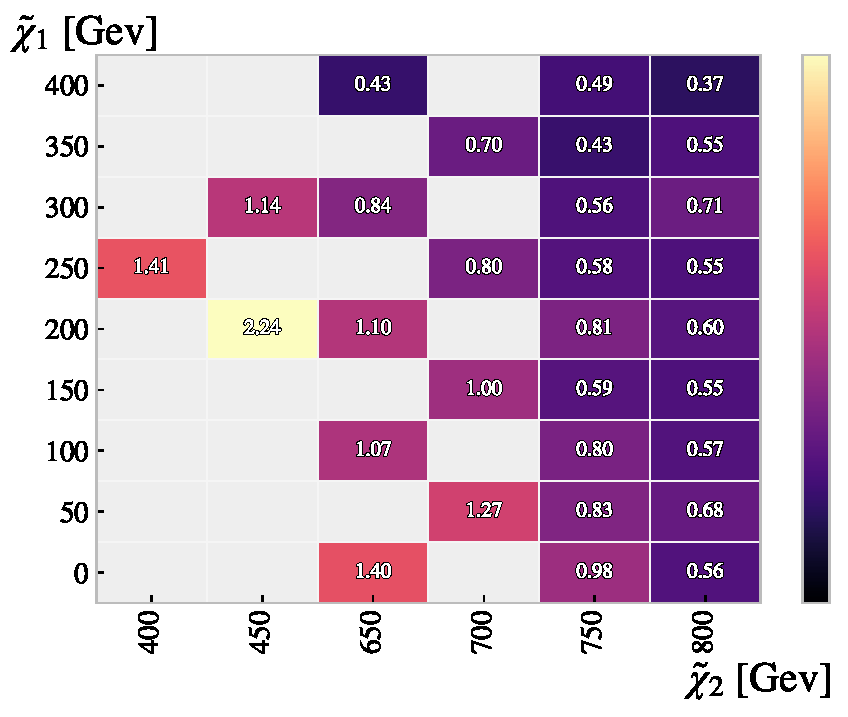
\includegraphics[width=\textwidth]{Figures/MLResults/NN/SUSY/Grid/StochChannelOutGridSig.pdf}
        \vspace{-1cm}
        \caption{}
        \label{fig:StochChannelOutGridSig}
    \end{subfigure}
    \begin{subfigure}{.5\textwidth}
        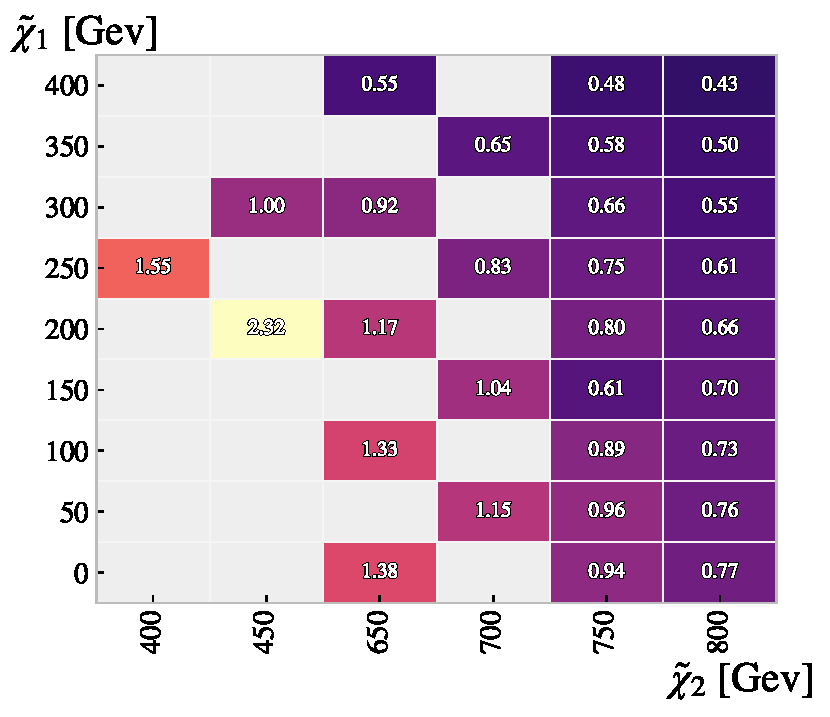
\includegraphics[width=\textwidth]{Figures/MLResults/NN/SUSY/Grid/ChannelOutGridSig.pdf}
        \vspace{-1cm}
        \caption{}
        \label{fig:ChannelOutGridSig}
    \end{subfigure}
    }
    \caption{A grid displaying the expected significance on the original signal set, using the signal region 
    created by the \acs{SCO} \ref{fig:StochChannelOutGridSig} and a channel-out network \ref{fig:ChannelOutGridSig}.}
    \label{fig:SCOCO}
\end{figure}

\subsection{Results from the \ac{PCA}}\label{appendix:PCA}
\begin{figure}[H]
    \makebox[\linewidth][c]{%
    \centering
    \begin{subfigure}{.5\textwidth}
        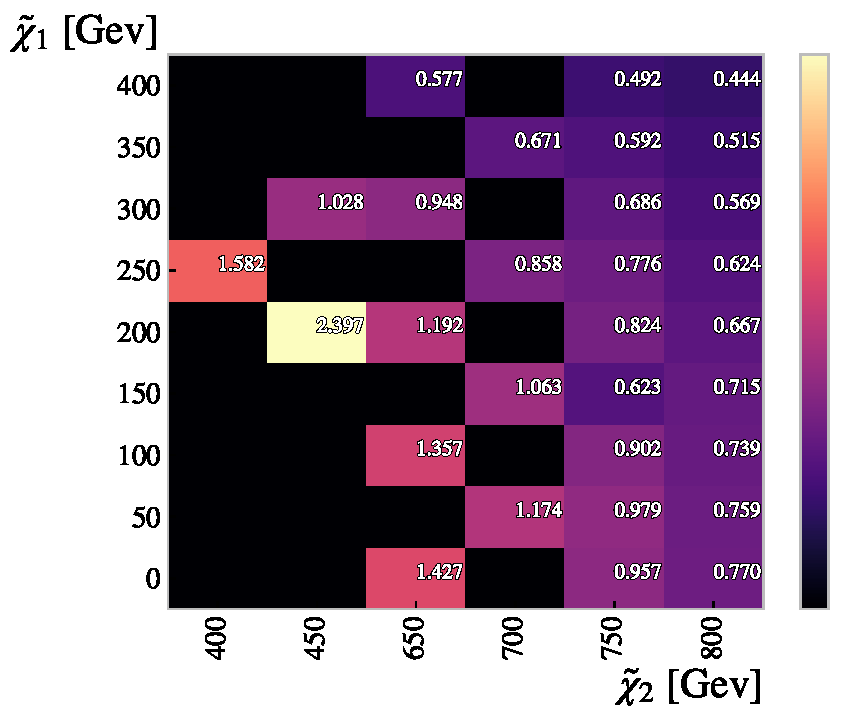
\includegraphics[width=\textwidth]{Figures/MLResults/NN/SUSY/Grid/NNPCAGridSig.pdf}
        \caption{}
        \label{fig:NNPCAGridSig}
    \end{subfigure}
    \begin{subfigure}{.5\textwidth}
        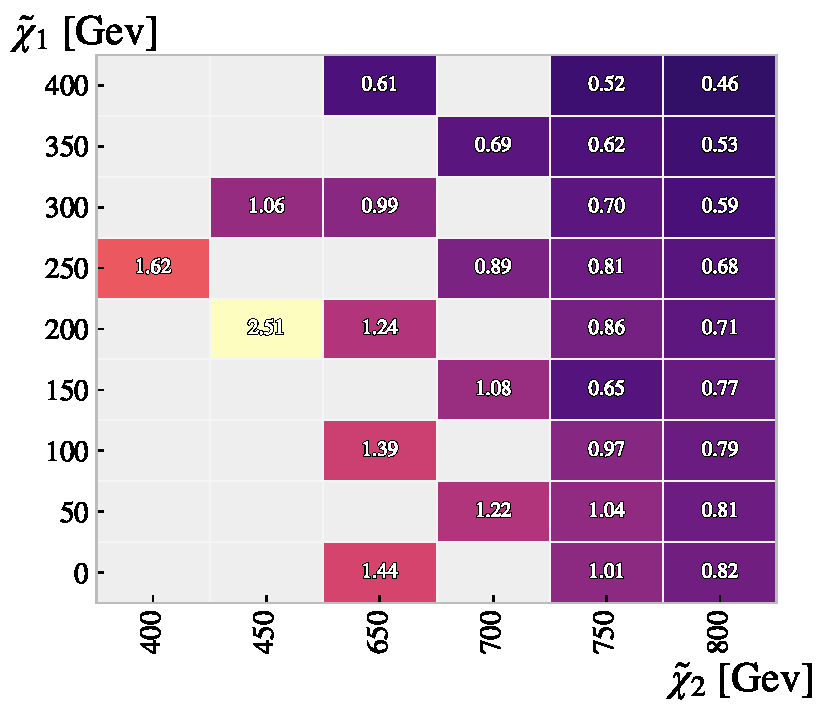
\includegraphics[width=\textwidth]{Figures/MLResults/NN/SUSY/Grid/MaxOutPCAGridSig.pdf}
        \caption{}
        \label{fig:MaxOutPCAGridSig}
    \end{subfigure}
    }
    \caption{A grid displaying the expected significance on the original signal set, using the signal region 
    created by the \acs{NN} \ref{fig:NNPCAGridSig} and a maxout network \ref{fig:MaxOutPCAGridSig}. A \ac{PCA} 
    analysis has been applied to the data being utilized in this result.}
\end{figure}

\begin{figure}[H]
    \makebox[\linewidth][c]{%
    \centering
    \begin{subfigure}{.65\textwidth}
        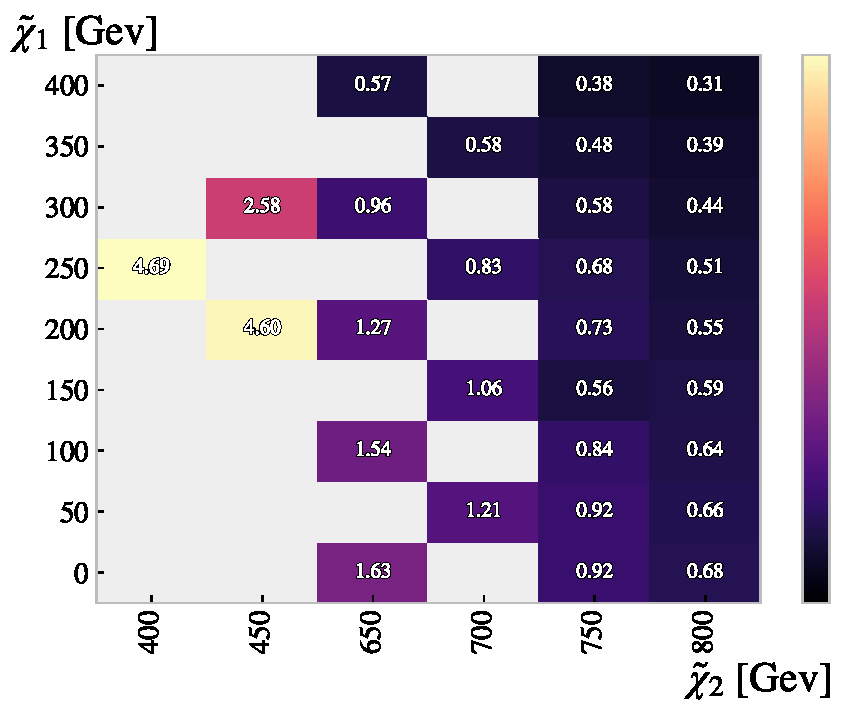
\includegraphics[width=\textwidth]{Figures/MLResults/NN/SUSY/Grid/PNNPCAGridSig.pdf}
    \end{subfigure}
    }
    \caption{A grid displaying the expected significance on the original signal set, using the signal region 
    created by the \acs{PNN} network. A \acs{PCA} analysis has been applied to the data being utilized in this result.}
    \label{fig:PNNPCAGridSig}
\end{figure}

\begin{figure}[H]
    \makebox[\linewidth][c]{%
    \centering
    \begin{subfigure}{.65\textwidth}
        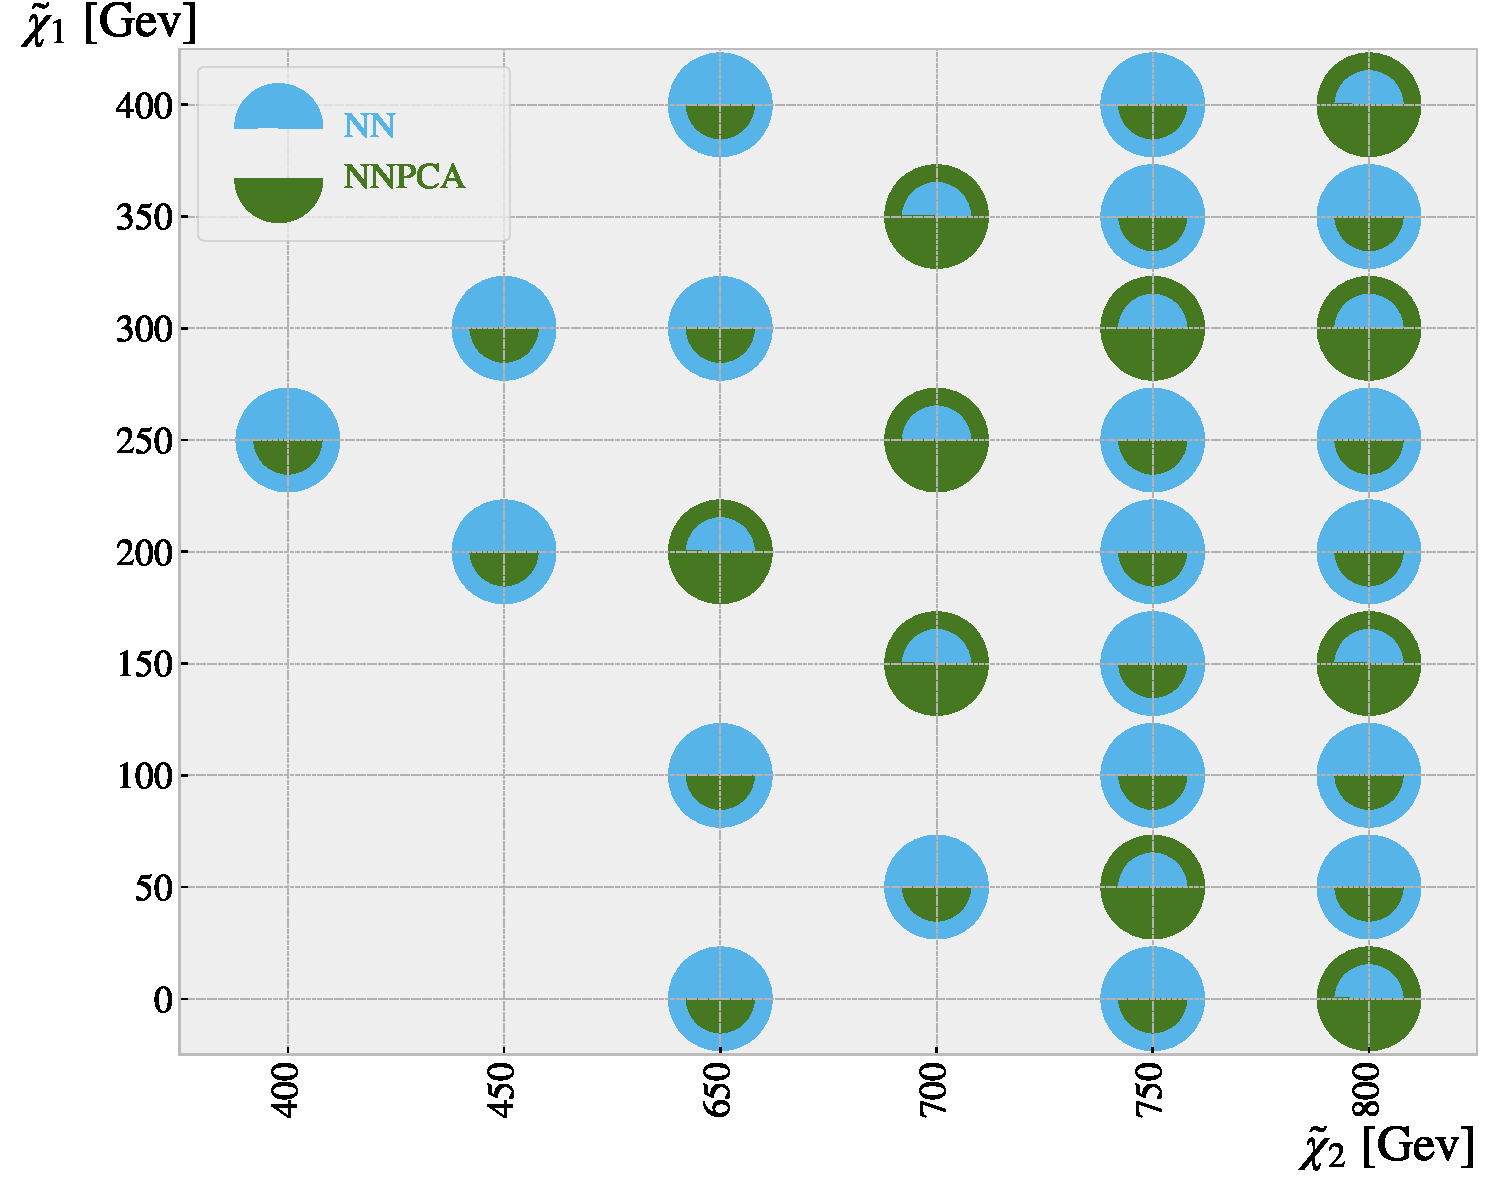
\includegraphics[width=\textwidth]{Figures/MLResults/NN/SUSY/Comparison/NNPCANetworkComp.pdf}
    \end{subfigure}
    }
    \caption[Pie-plot comparing sensitivity on the original signal set, where the figure shows the comparison between a model training on data 
    with and without a \acs{PCA}.]{Pie-plot comparing sensitivity on the original signal set, where the figure shows the comparison between a model trained on data 
    with and without a \acs{PCA}. The size of each 'slice' represents the relative size of the significance and the color around each 
    point displays the method with the largest sensitivity for the respective combination.}
    \label{fig:NNPCAComp}
\end{figure}

\subsection{Comparing Models Trained on Original and the Complete Signal Grid}\label{appendix:BigVsSmall}
\begin{figure}[H]
    \makebox[\linewidth][c]{%
    \centering
    \begin{subfigure}{.65\textwidth}
        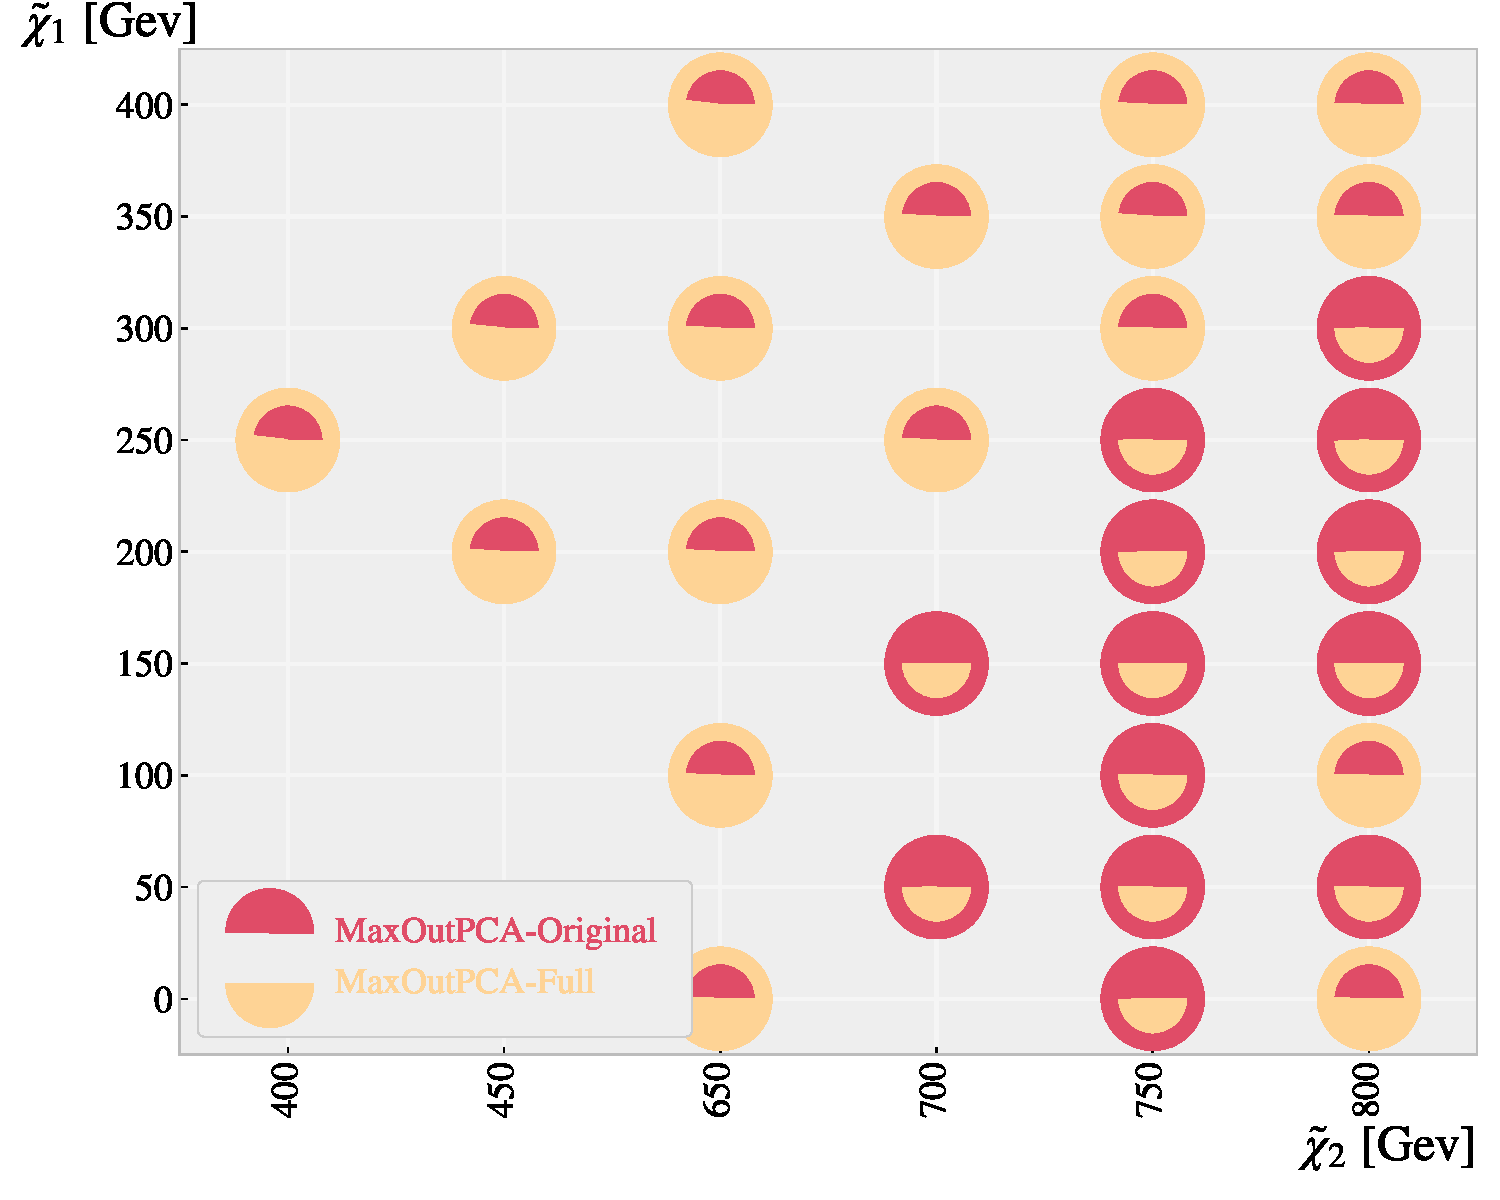
\includegraphics[width=\textwidth]{Figures/MLResults/NN/SUSY/Comparison/BigVsLittleSetMaxOutNetworkComp.pdf}
    \end{subfigure}
    }
    \caption[Pie-plot comparing sensitivity achieved by the maxout model on the original signal set, where the figure shows the comparison between a model trained 
    on the original signal grid, and the complete signal grid.]{Pie-plot comparing sensitivity achieved by the maxout model on the original signal set, where the figure 
    shows the comparison between a model trained on the original signal grid, and the complete signal grid.. A \ac{PCA} analysis has been applied to the data being utilized 
    in this result. The size of each 'slice' represents the relative size of the significance and the color around each 
    point displays the method with the largest sensitivity for the respective combination.}
    \label{fig:BigVsLittleSetMaxOut}
\end{figure}
\begin{figure}[H]
    \makebox[\linewidth][c]{%
    \centering
    \begin{subfigure}{.65\textwidth}
        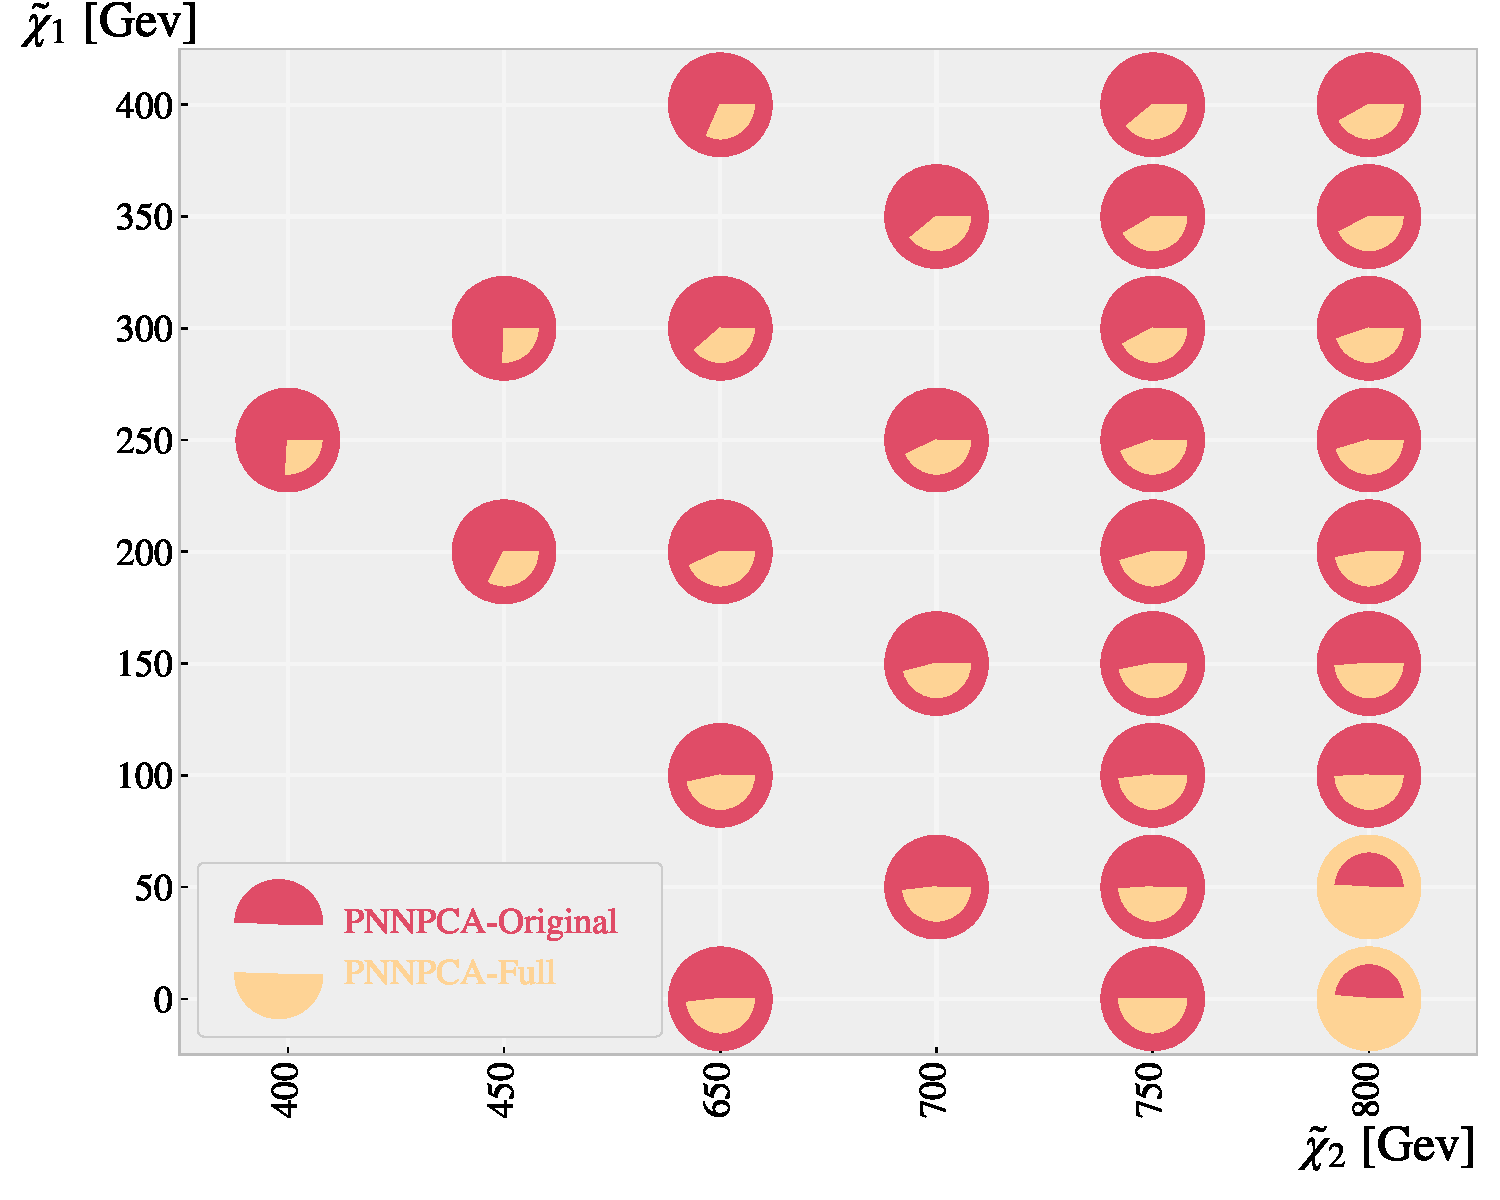
\includegraphics[width=\textwidth]{Figures/MLResults/NN/SUSY/Comparison/BigVsLittleSetPNNNetworkComp.pdf}
    \end{subfigure}
    }
    \caption[Pie-plot comparing sensitivity achieved by the \acs{PNN} model on the original signal set, where the figure shows the comparison between a model trained 
    on the original signal grid, and the complete signal grid.]{Pie-plot comparing sensitivity achieved by the \acs{PNN} model on the original signal set, where the figure 
    shows the comparison between a model trained on the original signal grid, and the complete signal grid. A \ac{PCA} analysis has been applied to the data being utilized 
    in this result. The size of each 'slice' represents the relative size of the significance and the color around each 
    point displays the method with the largest sensitivity for the respective combination.}
    \label{fig:BigVsLittleSetPNN}
\end{figure}
\newpage